

\hspace{4mm} La modélisation a pour objectif de formaliser les étapes préliminaires du développement d'un système afin de répondre aux besoins fixés dans la spécification du système. 
\par Dans ce chapitre nous détaillons les points forts de l’UML, par la suite nous présentons une conception détaillée pour bien comprendre la structure de notre projet. 
\section{	Architecture de l'application  }

\hspace{4mm} Afin de simplifier la mise à jour de l’application et d’en faciliter l’accès, le futur système va être développé sur la base d’une application Web. Une application Web se trouve sur un serveur et se manipule à l'aide d'un navigateur Web (Chrome, Firefox, …), via un réseau informatique (Internet, intranet, réseau local, etc.). Dans la technologie client-serveur, utilisée pour le World Wide Web, la communication est organisée par l'intermédiaire d'un réseau et d'une interface Web entre plusieurs ordinateurs." cela signifie que des machines clientes (machines faisant partie du réseau) contactent un serveur, une machine généralement très puissante en termes de capacités d'entrées-sorties, qui leur fournit des services. Ces services sont exploités par des programmes, appelés programmes clients, s'exécutant sur les machines clientes."\cite{12}.  
\par L'application Web s'oriente autour d'un serveur Web sur lequel est branché le logiciel applicatif, le tout accompagné d'un serveur de base de données.  
\par 
	Un des principaux avantages d’une application Web est que son utilisation est totalement indépendante du matériel de l’utilisateur. Qu’il utilise un PC ou un autre environnement, l’utilisateur n'a besoin que d’un explorateur pour accéder au système.


\subsection{	Design pattern MVC    }


\hspace{4mm}Dans le souci de développer une application stable et évolutive, l’utilisation d’une architecture standardisée est primordiale. Le Design Pattern Model-View-Controller est l'une des techniques de codage les plus répandues, principalement dans le développement Web. Les nouvelles possibilités d’interfaçages riches apportent de nouveaux défis. Le pattern MVC offre la possibilité de créer des applications plus flexibles. 
\par Rassembler les vues et les données a plusieurs inconvénients : 
\begin{itemize}
    \item 	La difficulté de gérer les données de l’extérieur de l’objet. 
    \item	La difficulté de créer différentes interfaces utilisateurs. 
    \item 	La difficulté de faire évoluer les interfaces. 
\end{itemize}
\par  Le concept de base du pattern MVC repose sur la séparation des données et des vues dans des logiques différentes. Le pattern MVC est basé sur trois couches : 
\par\textbf{	Le modèle }

\par Il décrit ou contient les données manipulées par l'application. Dans le cas typique d'une base de données le modèle offre des méthodes pour mettre à jour ces données (insertion, suppression, changement de valeur). Il offre aussi des méthodes pour récupérer ces données. Les résultats renvoyés par le modèle sont dénués de toute présentation. C'est le modèle qui contient toute la logique métier de l'application \cite{2}. 
\par\textbf{	La vue  }

\par La vue correspond à l'interface avec laquelle l'utilisateur interagit. Sa première tâche est de présenter les résultats renvoyés par le modèle qui lui sont passés par le contrôleur. Sa seconde tâche est de recevoir toutes les actions de l'utilisateur (clic de souris, sélection d'une entrée, boutons, soumission de formulaires). Ces différents événements sont envoyés au contrôleur. La vue n'effectue aucun traitement, elle se contente d'afficher les résultats des traitements effectués par le modèle \cite{2}. 
\newpage \par \textbf{	Le contrôleur   }

\par Le contrôleur prend en charge la gestion des événements de synchronisation pour mettre à jour la vue ou le modèle et les synchroniser. Il reçoit tous les événements de l'utilisateur et dénclenche les actions à effectuer. Si une action nécessite un changement des données, le contrôleur demande la modification des données au modèle et ensuite avertit la vue que les données ont changé pour qu'elle se mette à jour \cite{2}.
\begin{figure}[h]
    \centering
    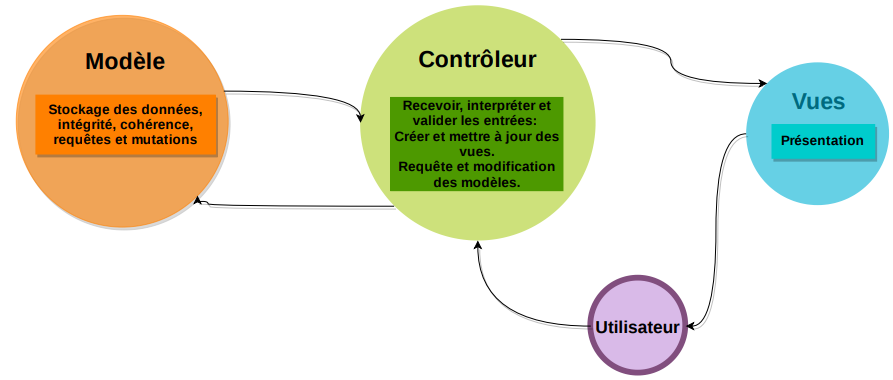
\includegraphics[scale=0.5]{figures/a11.png}
    \caption{Architecture MVC}
    \label{fig:Arch_MVC}
\end{figure}
\par En résumé, lorsqu'un client envoie une requête à l'application :
\begin{itemize}
    \item 	La requête est analysée par le contrôleur. 
    \item Le contrôleur demande au modèle approprié d'effectuer les traitements.
    \item 	Le contrôleur renvoie la vue adaptée. 
\end{itemize}

\subsection{	Backend Spring Boot avec Spring Security }
\hspace{4mm}Voici un diagramme pour les classes Spring Security / JWT qui sont séparées en 3 couches \cite{3}:
\begin{itemize}
    \item 	HTTP
    \item 	Spring Security
    \item 	REST API
\end{itemize}
\newpage
\begin{figure}[h]
    \centering
    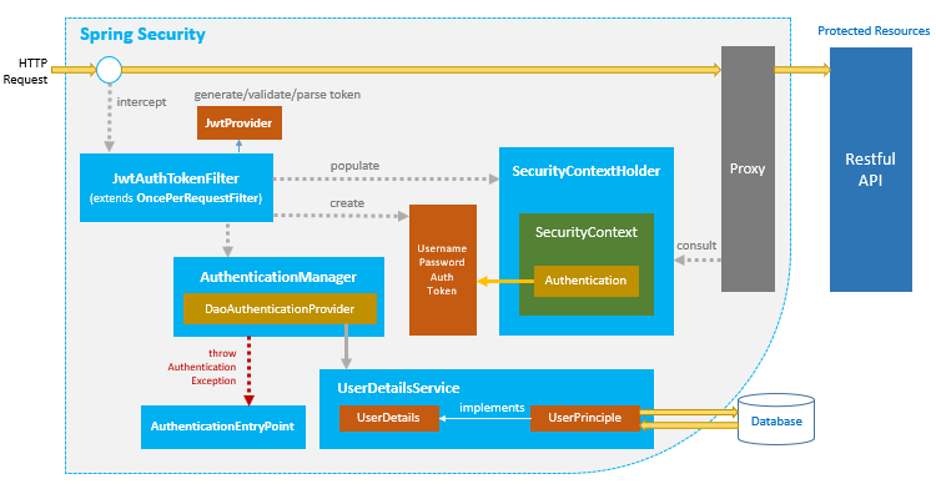
\includegraphics{figures/3anis1.png}
    \caption{Architecture Backend Spring Boot avec Spring Security \cite{3}}
    \label{fig:arch_backend}
\end{figure}
\begin{itemize}
    \item[-]\textbf{SecurityContextHolder} permet d'accéder au \textbf{SecurityContext}.
    \item[-] \textbf{SecurityContext} contient l'authentification et éventuellement les informations de sécurité spécifiques à la demande.
    \item[-]	L'authentification appelle \textbf{UserPrinciple} qui inclut \textbf{GrantedAuthority} qui reflète les autorisations à l'échelle de l'application accordée à \textbf{UserPrinciple}.
    \item[-]\textbf{UserDetails} contient les informations nécessaires pour créer un objet d'authentification à partir de DAO ou d'une autre source de données de sécurité.
    \item[-]\textbf{UserDetailsService} permet de créer un \textbf{UserDetails} à partir d'un nom d'utilisateur basé sur une chaîne et est généralement utilisé par \textbf{AuthenticationProvider}.
    \item[-]\textbf{JwtAuthTokenFilter} (étend \textbf{OncePerRequestFilter}) prétraite la requête HTTP, à partir de Token, crée une \textbf{Authentification} et la remplit dans \textbf{SecurityContext}.
    \item[-]\textbf{JwtProvider} valide, analyse la chaîne de jeton ou génère la chaîne de jeton à partir de \textbf{UserDetails}.
    \item[-]\textbf{UsernamePasswordAuthenticationToken} obtient l’email/ mot de passe de la demande de connexion et se combine dans une instance de l'interface d'authentification.
    \item[-]\textbf{AuthenticationManager} utilise \textbf{DaoAuthenticationProvider} (avec l'aide de \textbf{UserDetailsService et PasswordEncoder}) pour valider l'instance de \textbf{UsernamePasswordAuthenticationToken}, puis renvoie une instance d'authentification entièrement remplie en cas d'authentification réussie.
    \item[-]\textbf{SecurityContext} est établi en appelant \newline \textbf{SecurityContextHolder.getContext().SetAuthentication(…)} avec l'objet d'authentification renvoyé ci-dessus.
    \item[-]\textbf{AuthenticationEntryPoint} gère \textbf{AuthenticationException}.
    \item[-]L'accès à Restful API est protégé par HTTPSecurity et autorisé avec Method Security Expressions.
\end{itemize}
\subsection{	Front-end angular avec interceptor }
\hspace{4mm}La figure \ref{fig:arch_frontend} ci-dessous décrit l'architecture angular avec interceptor. \cite{4}
\begin{figure}[h]
    \centering
    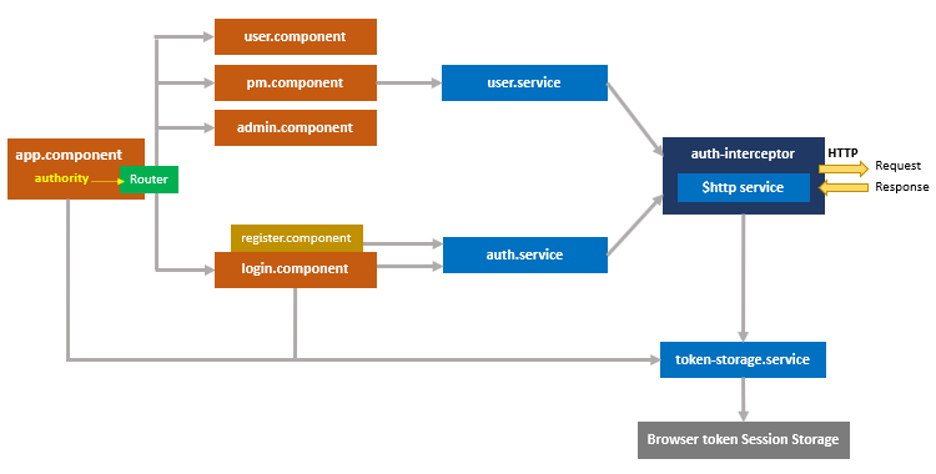
\includegraphics{figures/3anis2.png}
    \caption{Architecture Front-end angular avec interceptor \cite{4}}
    \label{fig:arch_frontend}
\end{figure}
\begin{itemize}
    \item[-]\textbf{app.component} est le composant parent qui contient \textbf{routerLink} et \textbf{router-outlet} pour le routage. Il a également une variable d'autorité comme condition d'affichage des éléments sur la barre de navigation. 
e    \item[-]\textbf{user.component, pm.component} et  \textbf{admin.component} correspondent à Angular Components for User Board, PM Board et Admin Board. Chaque conseil utilise \textbf{user.service} pour accéder aux données d'autorité.
    \item[-]\textbf{register.component} contient le formulaire d'inscription de l'utilisateur, la soumission du formulaire appellera \textbf{auth.service}.
    \item[-]\textbf{login.component} contient le formulaire de connexion utilisateur, la soumission du formulaire appellera \textbf{auth.service} et \textbf{token-storage.service}.
    \item[-]\textbf{user.service} obtient l'accès aux données d'autorité du serveur en utilisant Angular \textbf{HttpClient} (http service).
    \item[-]Chaque requête HTTP par le service \textbf{http} sera inspectée et transformée avant d'être envoyée au serveur par auth-interceptor (implements \textbf{HttpInterceptor}).
    \item[-]\textbf{auth-interceptor} vérifie et récupère le jeton depuis \textbf{token-storage.service} pour ajouter le jeton à l'en-tête d'autorisation des requêtes HTTP.
    \item[-]\textbf{token-storage.service} gère le jeton dans le sessionStorage du navigateur.
\end{itemize}
\subsection{	Architecture angular 9 et Spring Boot}
\hspace{4mm}La figure \ref{fig:spring_boot} ci-dessous décrit l'architecture angular et spring boot:
\begin{figure}[h]
    \centering
    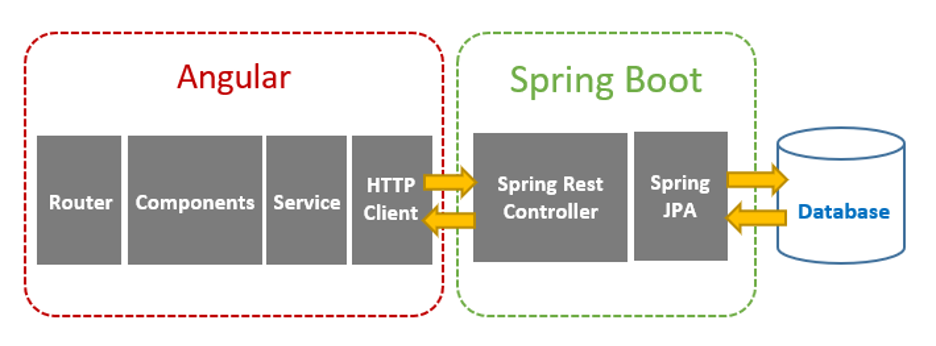
\includegraphics{figures/3anis3.png}
    \caption{Architecture angular 9 ET Spring Boot \cite{13}}
    \label{fig:spring_boot}
\end{figure}
\begin{itemize}
    \item	Spring Boot exporte les Apis REST à l'aide de Spring Web MVC et interagit avec la base de données à l'aide de Spring Data JPA.
    \item Angular Client envoie des requêtes HTTP, récupère des réponses HTTP et affiche des données sur les composants. Nous utilisons également Angular Router pour accéder aux pages.
    \item 	La base de données est PostgreSQL.
\end{itemize}
\section{Conception détaillée}
\subsection{	Diagrammes de classes }
\subsubsection{	Diagramme de classes global}
\hspace{4mm}Les classes font partie de la logique de l’application. Elles présentent non seulement la structure statique, mais aussi les différentes entités qui sont invoquées dans la conception de notre application. La figure \ref{fig:class_global} suivante présente le diagramme de classes que nous avons utilisé tout au long de ce projet. Les classes que nous avons créées dans ce projet correspondent à celles qui sont colorées dans la figure ci-dessous.
\par Dans la figure \ref{fig:class_global} on observe le diagramme de classe général en détails, à voir :
\begin{itemize}
    \item 	La classe : est un concept abstrait qui permet de représenter toutes les entités d'un système.
    \item	Les champs : ayant un type, pour distinguer le type de données à stocker pour ce champ.
    \item	La liaison d’héritage : Démarche ascendante, qui consiste à capturer les particularités communes d'un ensemble d'objets, issus de classes différentes.
    \item	La liaison d’agrégation : est une association non symétrique, qui exprime un couplage fort et une relation de subordination. Elle représente une relation de type "ensemble / élément".
    \item 	Les cardinalités de chaque liaison : selon le besoin, on distingue trois types de cardinalité sous django : 
    \begin{itemize}
        \item  ManyToMany relation : relation forte.
        \item  ManyToOne relation : relation moyenne
        \item  OneToOne relation : relation faible
    \end{itemize}
\end{itemize}


\begin{figure}
    \centering
    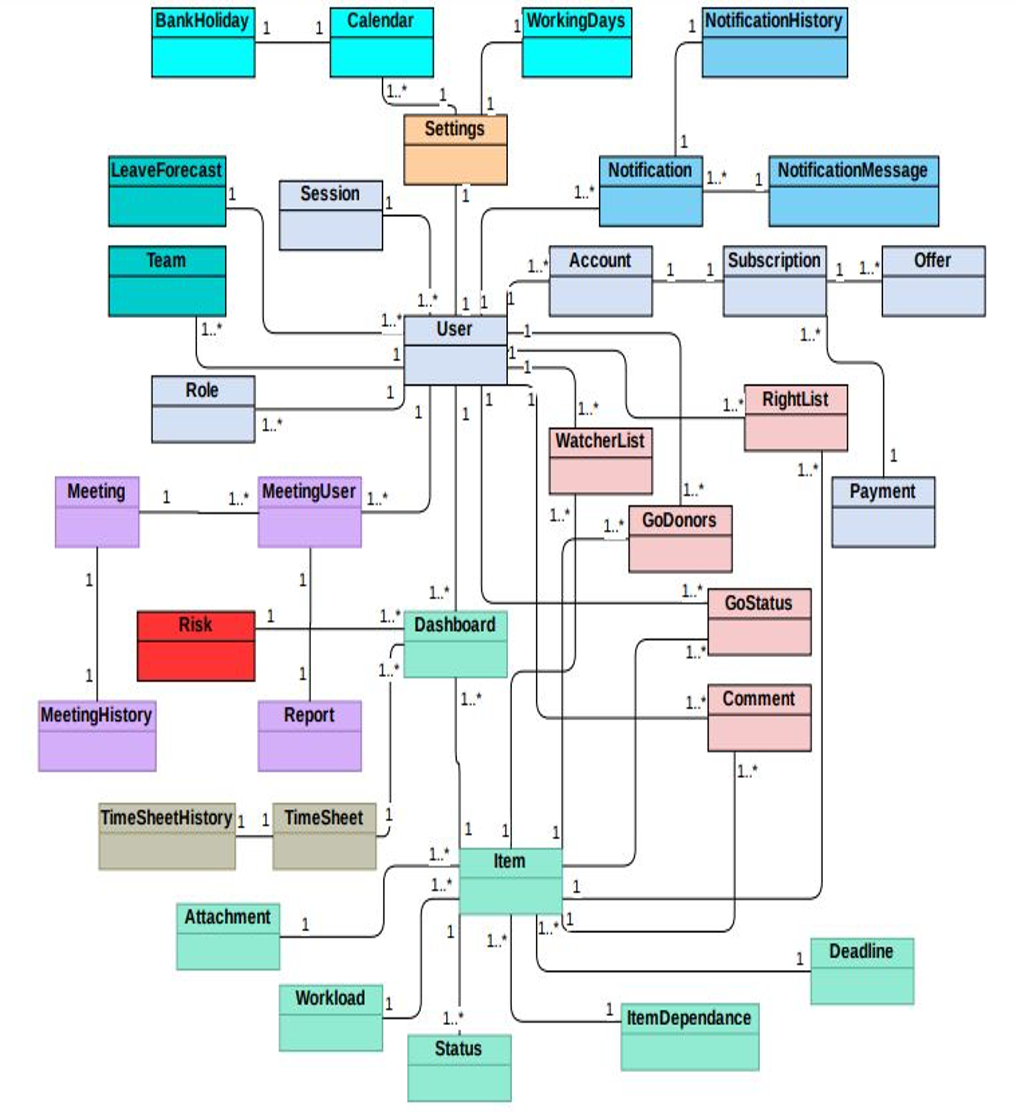
\includegraphics{figures/33anis.png}
    \caption{Diagramme de classes globale}
    \label{fig:class_global}
\end{figure}
\newpage
\subsubsection{	Diagramme de classes «Inscription et Authentification  »}
\hspace{4mm}Dans le diagramme de la figure \ref{fig:class_auth} on détaille les classes ainsi que les liaisons entre elles  pour la partie inscription et authentification.
\begin{itemize}
    \item 	Avant de s’inscrire (soumission des données d’un formulaire d’inscription) un objet de la classe \textbf{Session} est crée, il fournit en plus de son Id  un Token qui sera renvoyé par la suite à l’utilisateur dans le but de vérifier le statut de l’utilisateur (\textbf{status} :" True " peut se connecter, " False " connexion au compte impossible) avec un attribut lastConnection précisant un délai pour lequel le Token est valable.
    \item 	Saisie d’une offre : l’utilisateur choisit une offre de son choix tout en précisant le type de payement.  
\end{itemize}
\begin{figure}[h]
    \centering
    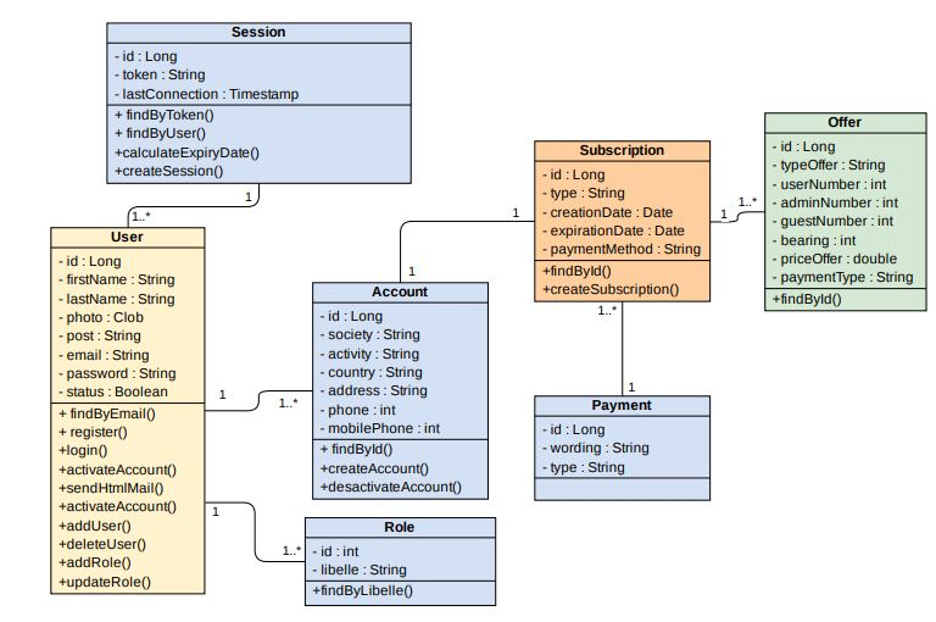
\includegraphics{figures/33Anis1.png}
    \caption{Diagramme de classes « Inscription et Authentification  »}
    \label{fig:class_auth}
\end{figure}\newpage
\subsubsection{Diagramme de classes « Gestion des Réunions, Notifications, Équipe et Paramétrage  »}
\begin{itemize}
    \item \textbf{Réunions} : En plus des détails des \textbf{Meeting} on trouve la classe \textbf{MeetingHistory} qui sert pour le traçage  des anciennes réunions établies via la plateforme ainsi qu’une classe Report qui permettra d’obtenir un compte Rendu de la réunion.
    \item \textbf{Notifications}: le contenu de la notification est récupéré par la classe \textbf{NotificationMessage}. Toute notification admet un statut et dispose d’un historique.
    \item \textbf{Paramétrage} : le paramétrage permet de donner les jours des travaux (on trouve les jours de la semaine qui sont bien partitionnés). On peut préciser les jours de congé en suivant la classe calendrier.
	\item\textbf{Équipe} : un utilisateur peut appartenir à une équipe.
\end{itemize}\newpage
\begin{figure}[h]
    \centering
    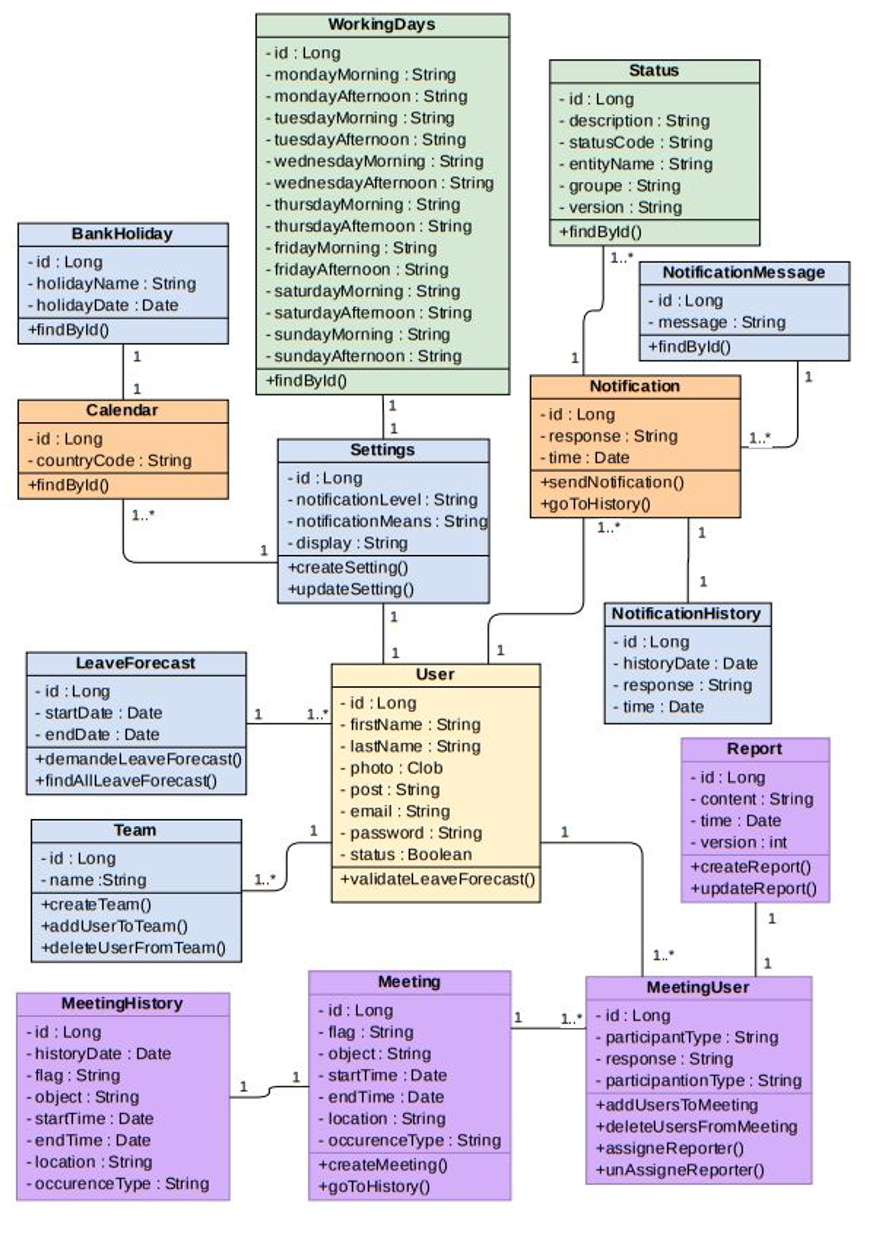
\includegraphics[scale=0.83]{figures/33anis2.png}
    \caption{Diagramme de classes «Gestion des Réunions, Notifications, Équipe et Paramétrage»}
    \label{fig:class_P2}
\end{figure}\newpage
\subsubsection{Diagramme de classes « Gestion de Projet »}
\hspace{4mm}Le diagramme de classes de la figure \ref{fig:class_P3} illustre toutes les entités indispensables à la gestion de projet. 
\begin{figure}[h]
    \centering
    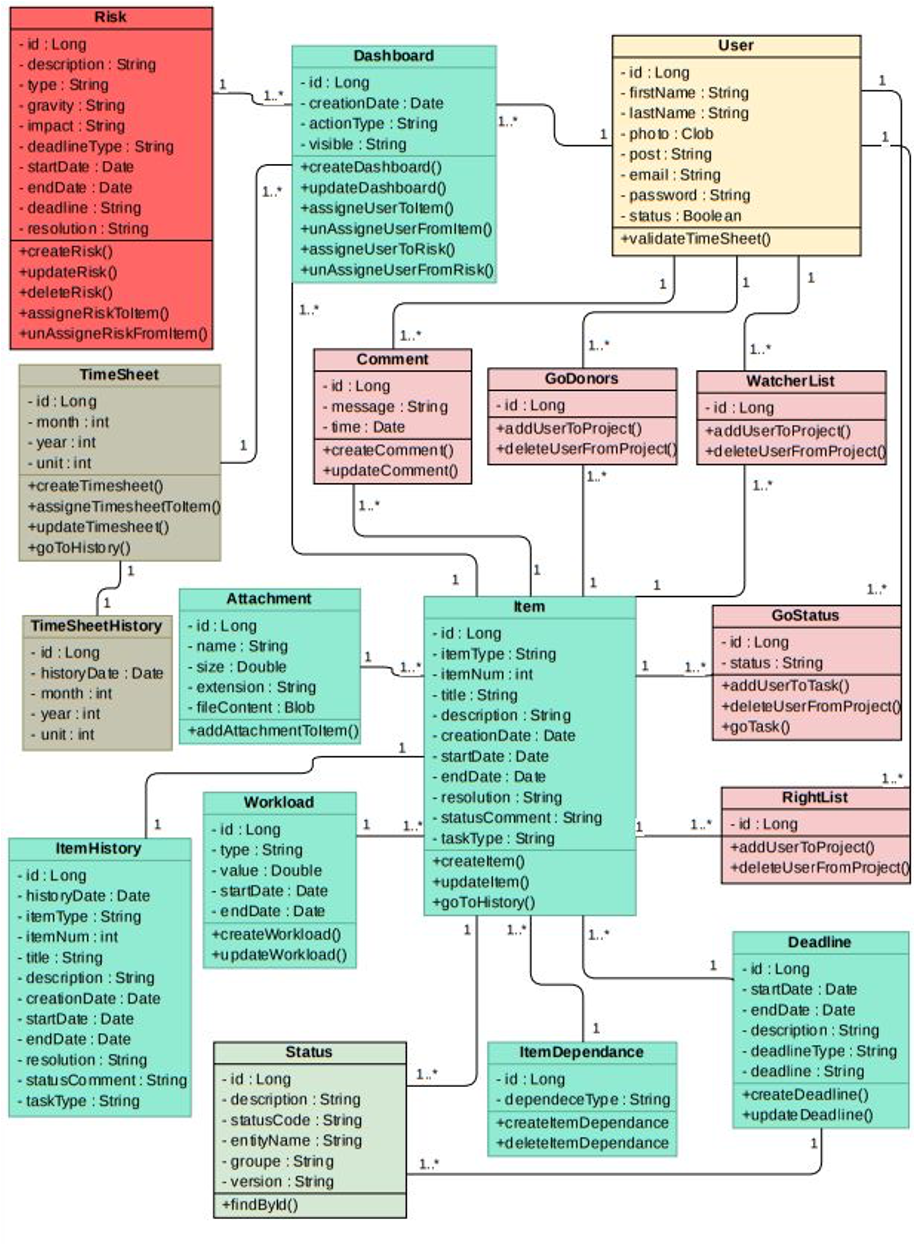
\includegraphics[scale=0.84]{figures/33anis3.png}
    \caption{Diagramme de classes « Gestion de Projet »}
    \label{fig:class_P3}
\end{figure}\newpage
\subsection{	Diagrammes de séquence }
\hspace{4mm}Le diagramme de séquence est une représentation séquentielle du déroulement des traitements et des interactions entre les éléments du système et/ou de ses acteurs \cite{14}. Avant d'entrer au menu du projet et faire l'ensemble des autres scénarios l'utilisateur doit se connecter. Le diagramme qui suit présente l'enchainement de la phase d'authentification. 
\newpage\par \textbf{	Authentification }
\begin{figure}[h]
    \centering
    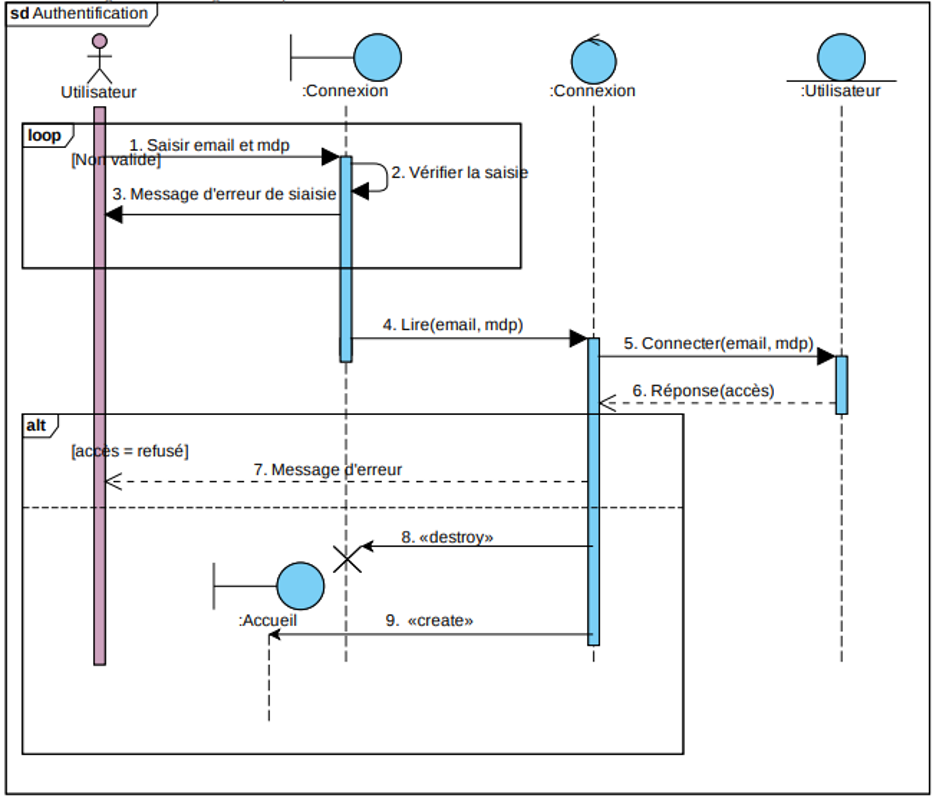
\includegraphics{figures/3anis5.png}
    \caption{Diagramme de Séquence " authentification "}
    \label{fig:Séquence_authentification}
\end{figure}
\par Description : 
\begin{itemize}
    \item L’utilisateur saisit son login et mot de passe pour accéder au système. Si les données introduites sont erronées, la page d’authentification se relance, sinon la page d’accueil du système s’ouvre.
\end{itemize}
\newpage\par \textbf{	Souscription  }
\begin{figure}[h]
    \centering
    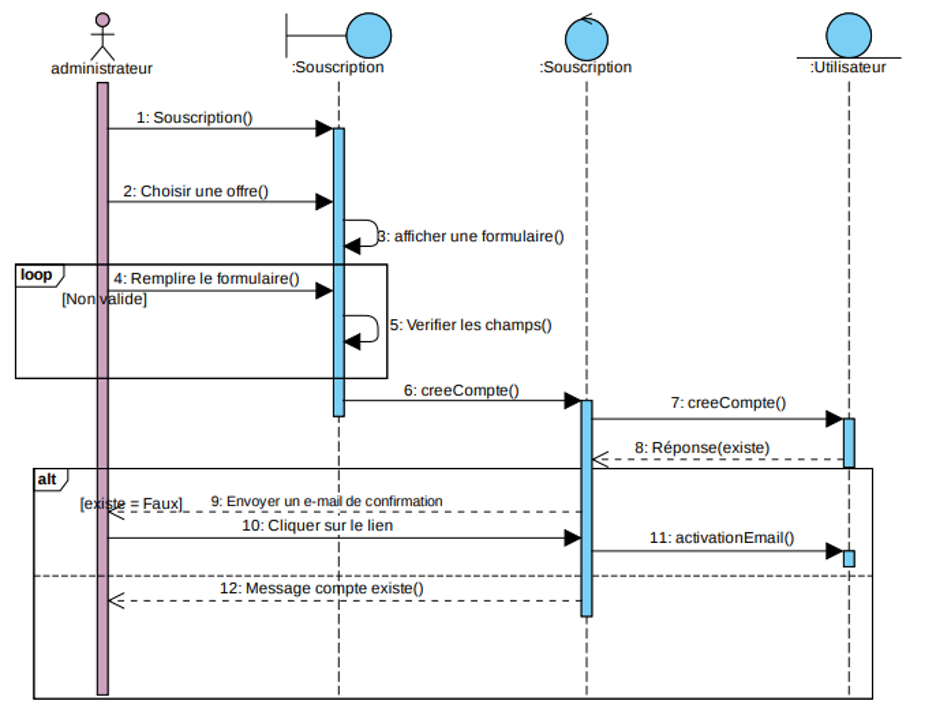
\includegraphics{figures/3anis6.png}
    \caption{Diagramme de Séquence " souscription "}
    \label{fig:Séquence_souscription}
\end{figure}
\par Description : 
\begin{itemize}
    \item L’utilisateur demande la souscription : une page s’affiche pour choisir une offre, selon l’offre choisie un formulaire à remplir s'affiche. Le système fait une vérification sur les champs, si tout est correct il envoie une requête d’inscription sinon un message d’erreur s’affiche sur les champs incorrects. Puis, selon les données saisies l'existence de ce compte est vérifié, si l’email existe un message d’erreur s’affiche, sinon les données seront enregistrées. 
\end{itemize}
\newpage\par \textbf{	Organiser une réunion   }
\begin{figure}[h]
    \centering
    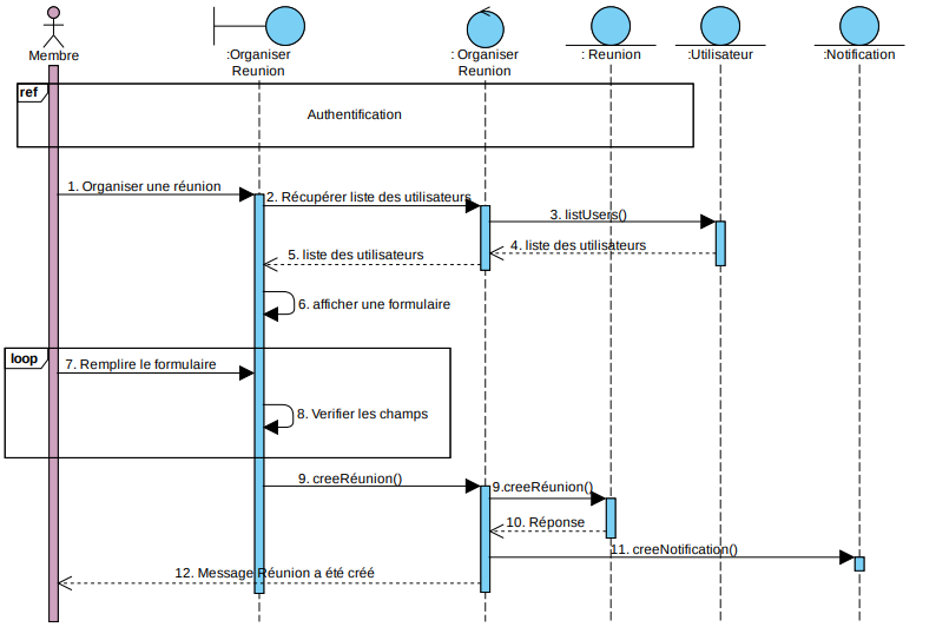
\includegraphics{figures/3anis7.png}
    \caption{Diagramme de Séquence "organiser une réunion"}
    \label{fig:Séquence_organiser}
\end{figure}
\par Description : 
\begin{itemize}
    \item 	L’utilisateur doit être authentifié pour organiser une réunion : un formulaire à remplir s'affiche. Il contient une liste des utilisateurs récupérée pour choisir les participants à la réunion. Le système fait une vérification sur les champs, si tout est correct il envoie une requête de création de réunion sinon un message d’erreur s’affiche sur les champs incorrects. Enfin, la réunion va être créée et selon les données saisies une notification sera envoyée à tous les participants.  
\end{itemize}
\section*{	Conclusion}
\hspace{4mm} 
Dans ce chapitre, nous avons présenté la conception de notre système. Nous avons détaillé l’architecture logiciel et nous avons établi le diagramme de classes et quelques diagrammes de séquences. Dans le dernier chapitre nous passerons à la phase de réalisation de tout ce qui a été défini et conçu tout au long des parties précédentes.


